\chapter{Results}
\label{Chapter5}
The CTF challenge was successfully implemented and deployed as described above: it's already available and 100\% functional, provided the web server is launched beforehands and the remote board is accessible.
Testing can be done by connecting to \url{http://130.192.93.82:8080/}, and the minimal form flag was found by means of the \emph{flag\_main.cpp} C++ script (located in the ``VHDL/'' directory):
\newline\textbf{00010001000100010001000100010001000100010001000100010000000000000000000000000}
\newline\textbf{00000000000000000000000000000010001000100010001000100010001000100010001000100}
\newline\textbf{01000000000000000000000000000000000000000000000000000000010001000100010001000}
\newline\textbf{1000100010001000100010001\textsubscript{2}} or equally \textbf{1111111111111000000000000011111111111110000}
\newline\textbf{000000000111111111111\textsubscript{16}}.

\textcolor{red}{Be careful when copy-pasting these values directly into the online webpage, as they include whitespaces and newline characters in order to properly fit into the portrait page layout of this PDF file!}
\begin{figure}[!ht]
\vspace{0.5cm}
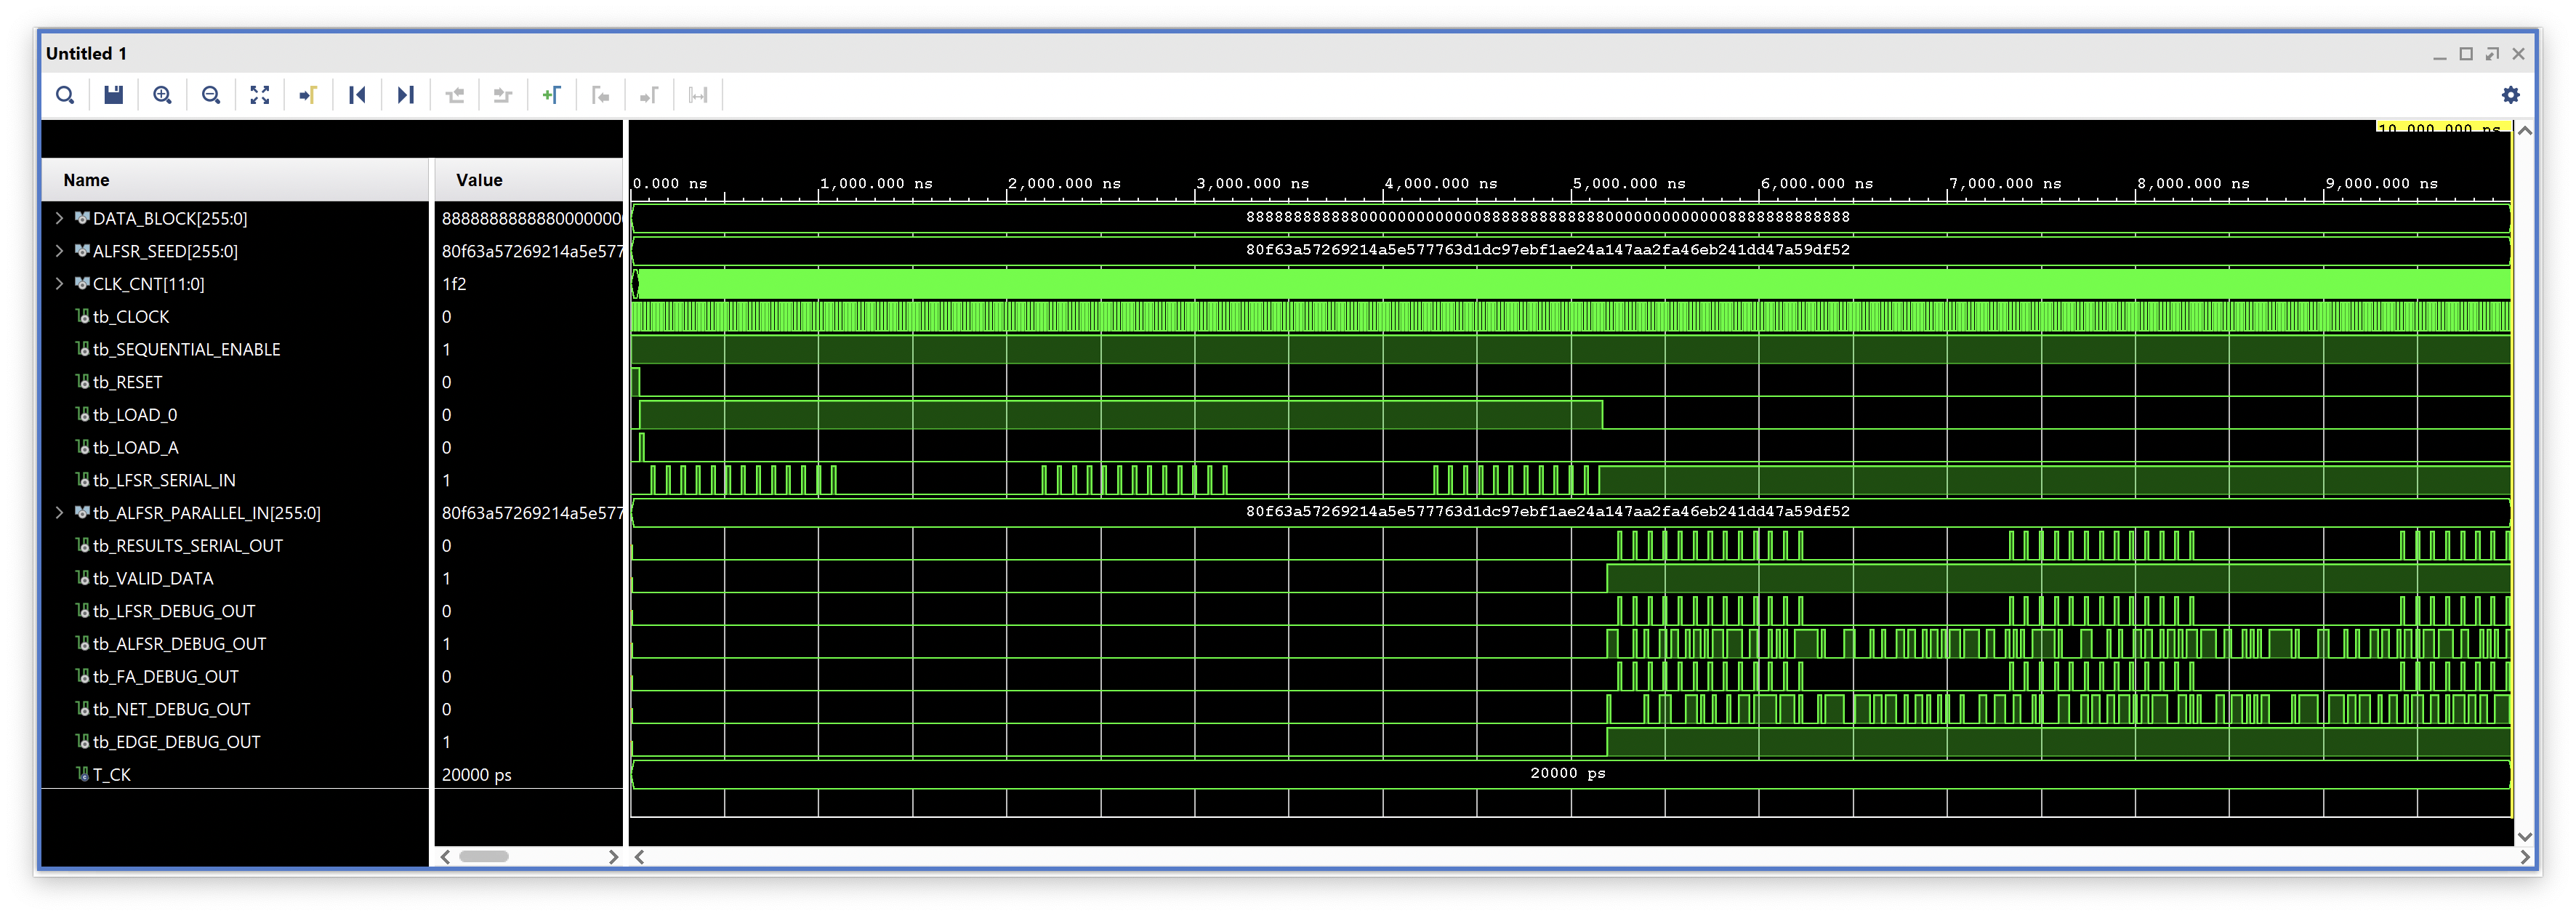
\includegraphics[width=\textwidth]{images/Waves.png}
\caption{Simulation of the vulnerability being triggered.}
\end{figure}
\section{Known Issues}
There are no known issues for the current state of the project, so this section is devoted to listing the differences between the initial demo and the final version instead:
\begin{itemize}
    \item The favicon of the website was changed in order to be aligned with the one found on the official website of the \emph{Politecnico di Torino} institute
    \item The `Reset' button was removed from the GUI, as its functionality gets implicitly called every time the user presses `Send' instead.
    The initial idea was to have the possibility of loading the plaintext with one or more breaks before reaching the acknowledge, as to leave the LFSR running and going through many more intermediate states.
    This concept was eventually scrapped as it didn't provide any substantial benefit to the complexity of the challenge, while creating many more implementation struggles and negatively impacting the synchronization side of the multi-user aspect
    \item The last screenshot of the original presentation included a preview of the \emph{EDGE.vhd} source file: the latter had to be totally reworked during the final stages of develompent, after some (tricky to detect) defects were discovered inside the the corresponding design.
\end{itemize}
\section{Future Work}
The provided web user interface will probably serve as more of a mockup, while the final challenge will have to be included within an official platform by the real organizers. This process will need to adhere to the instructions detailed in \autoref{api}.

Two possible improvements to the low-level design can also be discussed: the implementation of the `Reset' button, as described above, and the conception of a much more sophisticated vulnerability (produced by a real team of cybersecurity experts, for instance), referring to the enabler, the combinational network and the \emph{scrambler} components.